Consider the following Petri net:



\begin{centering}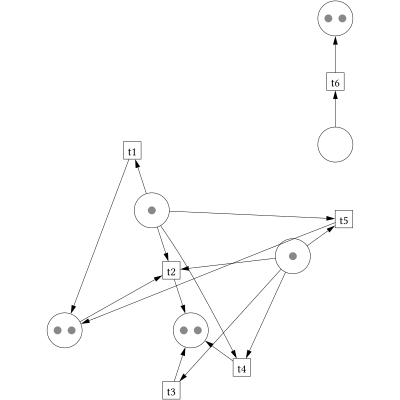
\includegraphics[min width=0.4\textwidth=0.6\textwidth,min height=0.4\textwidth=0.6\textwidth,keepaspectratio,max width=0.9\textwidth,max height=0.9\textwidth]{63/concurrentpetri7d70a8768ee1cdf2002c8d703dde2d744fda5473affcaeb8018a96c73a31bf8d01012.pdf}\end{centering}

Which pair of transitions is concurrently activated under the initial marking?

State your answer by giving a pair of concurrently activated transitions.  Stating \begin{verbatim}(t0,t1)\end{verbatim} as answer would indicate that transitions t0 and t1 are concurrently activated under the initial marking.  The order of transitions within the pair does not matter here.

Please note: When hovering over or clicking on edges / nodes or their labels, the respective components that belong together are highlighted.

